\noindent Linux Installation\textsuperscript{**}: Begin by ensuring that you have Virtual Box installed on your system, if not type:
\begin{lstlisting}[language=bash]
    $ sudo apt-get install virtualbox
\end{lstlisting}
%\vfill

%---------------------
\subsubsection{Create Virtual Machine}
\begin{figure}[!htb]
    \centering
    %\insertcode{Scripts/example.pl}{Nena would be proud.} % The first argument is the script location/filename and the second is a caption for the listing
    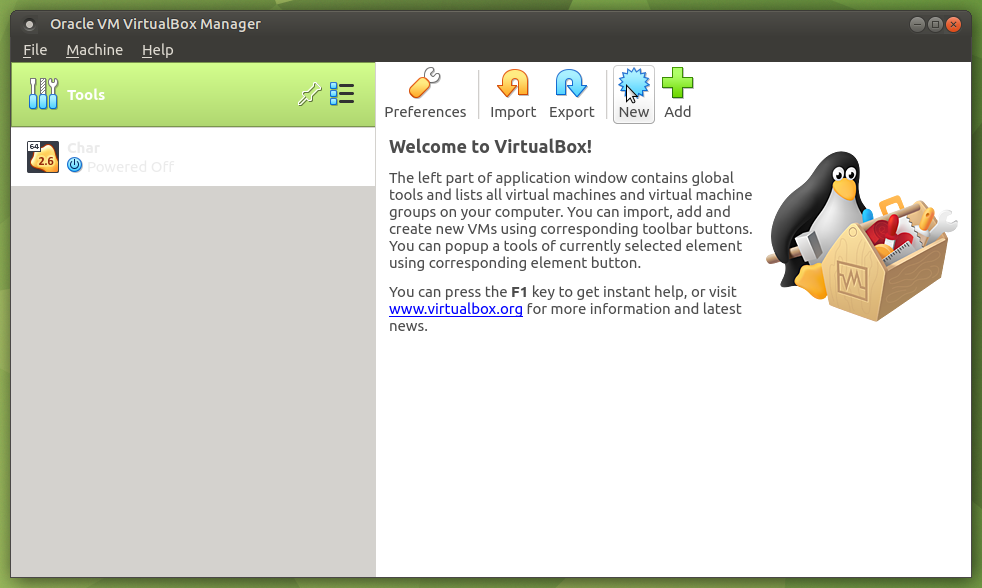
\includegraphics[width=0.752\textwidth]{images/00-0.png}\\[0cm]  
    \caption[Virtual Box]{New Virtual Machine Setup}
    %from \url{http://localhost:3000/}).} % The text in the square bracket is the caption for the list of figures while the text in the curly brackets is the figure caption
    \label{fig:00-01 - Linux Virtual Box New VM} 
\end{figure}
Begin by Creating a new Virtual Machine. To do this click on the blue icon
labelled new as shown in Figure \vref{fig:00-01 - Linux Virtual Box New VM}.

%---------------------
\subsubsection{Name \& Operating System}
\begin{figure}[!htb]
    \centering
    %\insertcode{Scripts/example.pl}{Nena would be proud.} % The first argument is the script location/filename and the second is a caption for the listing
    
\includegraphics[width=0.752\textwidth]{images/00-01.png}\\[0cm]  
    \caption[Virtual Box]{Setup Of Operating System Type and Name}
    \label{fig:00-02 - Linux Virtual Box Operating System} 
\end{figure}
You have to give your Virtual Machine a new name, I have chosen 'Darkly'. Make
sure to pick a folder for storage of the Virtual Machine or leave it to the
default provided by Virtual Box.

You will have to choose the 'type' of machine you are creating. At this point
you must select 'Linux' as this is what the Darkly.iso is based from. You will
be given options or 'flavours' to choose from. Pick 'Other 64-bit'. This is
shown in Figure ~\Vref{fig:00-02 - Linux Virtual Box Operating System}.

Please do take note that the Darkly VM will not work if it is not 64-bit.

%---------------------
\subsubsection{Memory Size}
\begin{figure}[!htb]
    \centering
    %\insertcode{Scripts/example.pl}{Nena would be proud.} % The first argument is the script location/filename and the second is a caption for the listing
    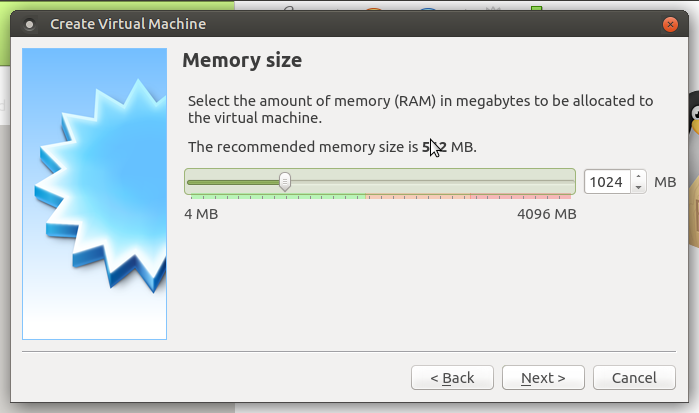
\includegraphics[width=0.752\textwidth]{images/00-02.png}\\[0cm]  
    \caption[Virtual Box]{Virtual Box Memory Size Settings}
    %from \url{http://localhost:3000/}).} % The text in the square bracket is the caption for the list of figures while the text in the curly brackets is the figure caption
    \label{fig:00-03 - Linux Virtual Box Memory Size} 
\end{figure}
Tell the system to use Linux

%---------------------
\subsubsection{Hard Disk File Type}
\begin{figure}[!htb]
    \centering
    %\insertcode{Scripts/example.pl}{Nena would be proud.} % The first argument is the script location/filename and the second is a caption for the listing
    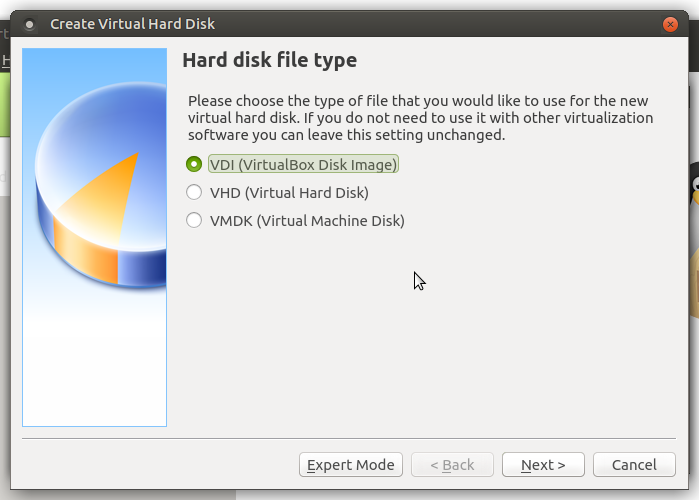
\includegraphics[width=0.752\textwidth]{images/00-03.png}\\[0cm]  
    \caption[Virtual Box]{\emph{Virtual Box Landing}, on Ubuntu}
    %from \url{http://localhost:3000/}).} % The text in the square bracket is the caption for the list of figures while the text in the curly brackets is the figure caption
    \label{fig:00-04 - Linux Virtual Box Landing} 
\end{figure}
Tell the system to use Linu

%---------------------
\subsubsection{Storage Type}

\begin{figure}[!htb]
    \centering
    %\insertcode{Scripts/example.pl}{Nena would be proud.} % The first argument is the script location/filename and the second is a caption for the listing
    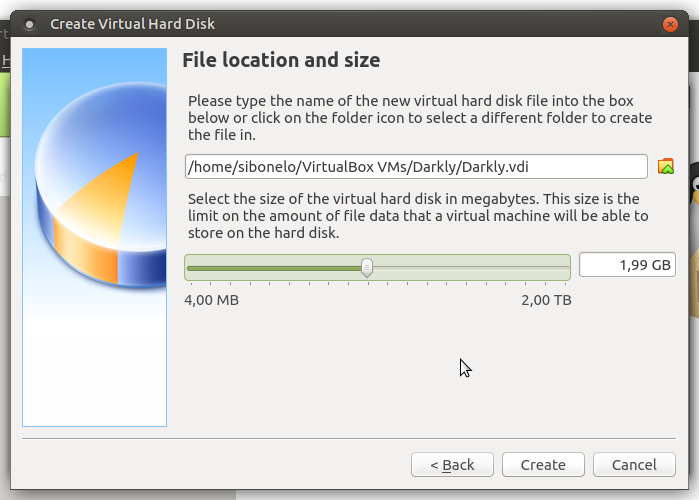
\includegraphics[width=0.752\textwidth]{images/00-05.png}\\[0cm]  
    \caption[Virtual Box]{\emph{Virtual Box Landing}, on Ubuntu}
    %from \url{http://localhost:3000/}).} % The text in the square bracket is the caption for the list of figures while the text in the curly brackets is the figure caption
    \label{fig:00-05 - Linux Virtual Box Landing} 
\end{figure}
Tell the system to use Linu

%---------------------
\subsubsection{File Location \& Size}

\begin{figure}[!htb]
    \centering
    %\insertcode{Scripts/example.pl}{Nena would be proud.} % The first argument is the script location/filename and the second is a caption for the listing
    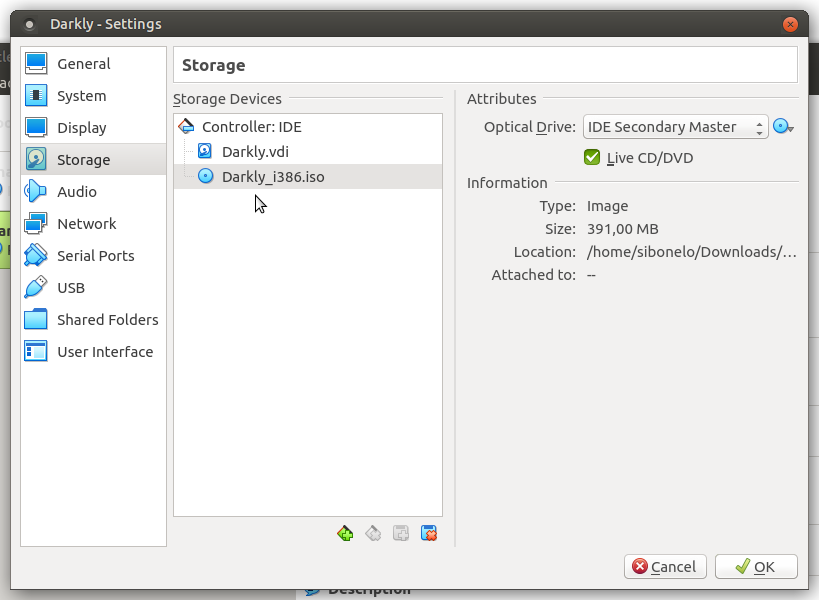
\includegraphics[width=0.752\textwidth]{images/00-06.png}\\[0cm]  
    \caption[Virtual Box]{\emph{Virtual Box Landing}, on Ubuntu}
    %from \url{http://localhost:3000/}).} % The text in the square bracket is the caption for the list of figures while the text in the curly brackets is the figure caption
    \label{fig:00-06 - Linux Virtual Box Landing} 
\end{figure}

Tell the system to use Linu
\subsubsection{Linux}

\begin{figure}[!htb]
    \centering
    %\insertcode{Scripts/example.pl}{Nena would be proud.} % The first argument is the script location/filename and the second is a caption for the listing
    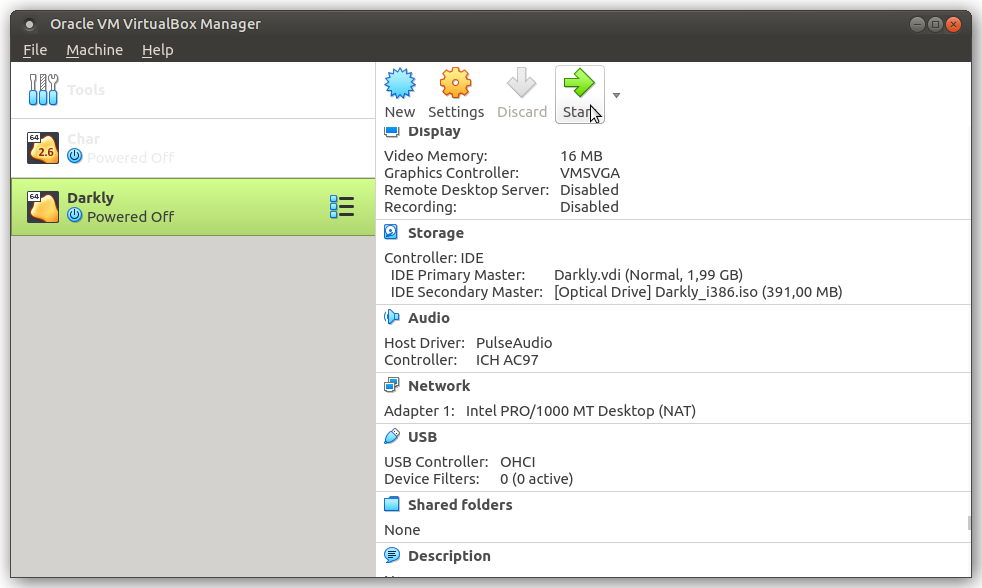
\includegraphics[width=0.752\textwidth]{images/00-07.png}\\[0cm]  
    \caption[Virtual Box]{\emph{Virtual Box Landing}, on Ubuntu}
    %from \url{http://localhost:3000/}).} % The text in the square bracket is the caption for the list of figures while the text in the curly brackets is the figure caption
    \label{fig:00-07 - Linux Virtual Box Landing} 
\end{figure}

Tell the system to use Linu
\subsubsection{Linux}

\begin{figure}[!htb]
    \centering
    %\insertcode{Scripts/example.pl}{Nena would be proud.} % The first argument is the script location/filename and the second is a caption for the listing
    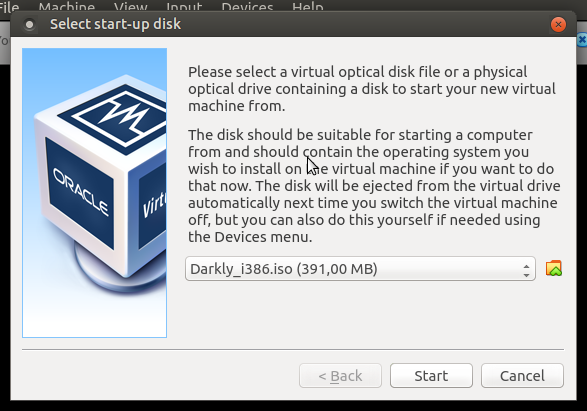
\includegraphics[width=0.752\textwidth]{images/00-08.png}\\[0cm]  
    \caption[Virtual Box]{\emph{Virtual Box Landing}, on Ubuntu}
    %from \url{http://localhost:3000/}).} % The text in the square bracket is the caption for the list of figures while the text in the curly brackets is the figure caption
    \label{fig:00-08 - Linux Virtual Box Landing} 
\end{figure}

Tell the system to use Linu
\subsubsection{Linux}

\begin{figure}[!htb]
    \centering
    %\insertcode{Scripts/example.pl}{Nena would be proud.} % The first argument is the script location/filename and the second is a caption for the listing
    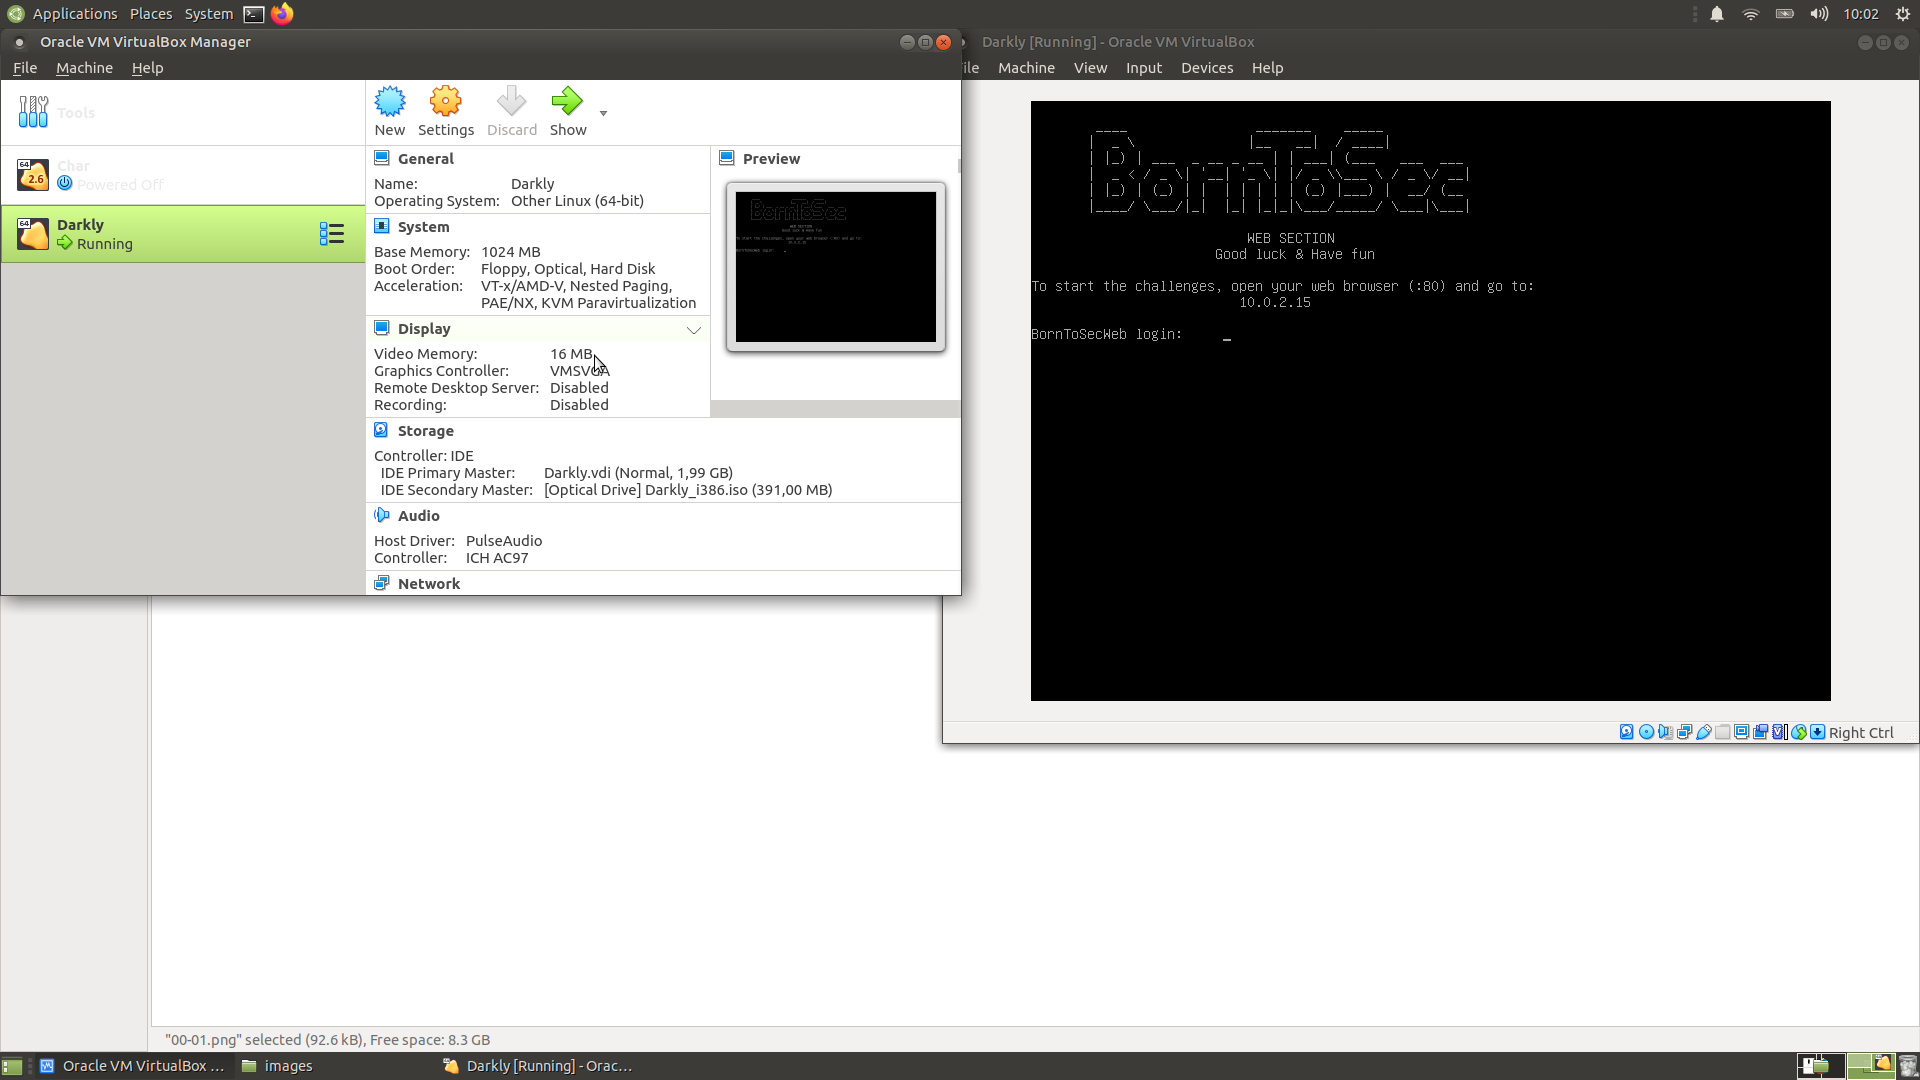
\includegraphics[width=0.752\textwidth]{images/00-09.png}\\[0cm]  
    \caption[Virtual Box]{\emph{Virtual Box Landing}, on Ubuntu}
    %from \url{http://localhost:3000/}).} % The text in the square bracket is the caption for the list of figures while the text in the curly brackets is the figure caption
    \label{fig:00-09 - Linux Virtual Box Landing} 
\end{figure}

Tell the system to use Linu
\subsubsection{Linux}

\begin{figure}[!htb]
    \centering
    %\insertcode{Scripts/example.pl}{Nena would be proud.} % The first argument is the script location/filename and the second is a caption for the listing
    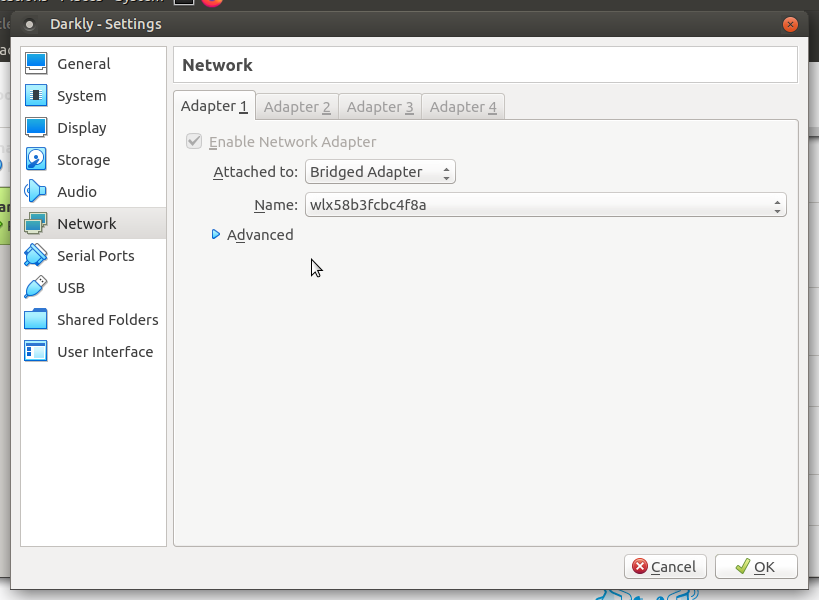
\includegraphics[width=0.752\textwidth]{images/00-10.png}\\[0cm]  
    \caption[Virtual Box]{\emph{Virtual Box Landing}, on Ubuntu}
    %from \url{http://localhost:3000/}).} % The text in the square bracket is the caption for the list of figures while the text in the curly brackets is the figure caption
    \label{fig:00-10 - Linux Virtual Box Landing} 
\end{figure}

Tell the system to use Linu
\subsubsection{Linux}

\begin{figure}[!htb]
    \centering
    %\insertcode{Scripts/example.pl}{Nena would be proud.} % The first argument is the script location/filename and the second is a caption for the listing
    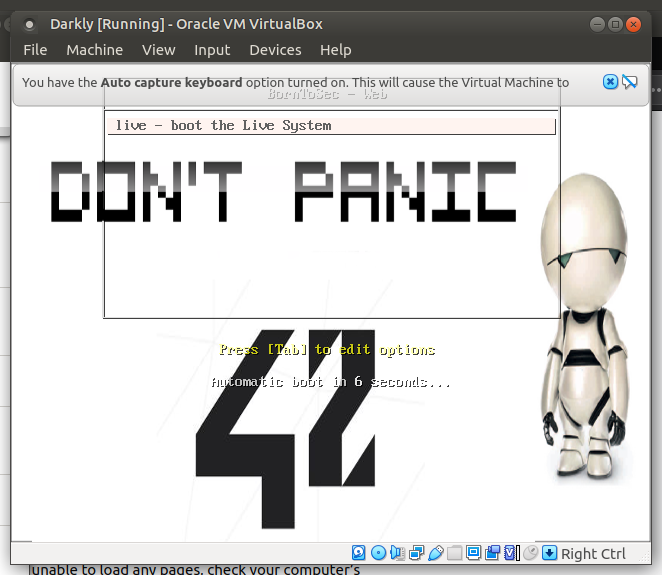
\includegraphics[width=0.752\textwidth]{images/00-11.png}\\[0cm]  
    \caption[Virtual Box]{\emph{Virtual Box Landing}, on Ubuntu}
    %from \url{http://localhost:3000/}).} % The text in the square bracket is the caption for the list of figures while the text in the curly brackets is the figure caption
    \label{fig:00-11 - Linux Virtual Box Landing} 
\end{figure}

Tell the system to use Linu

\subsubsection{Linux}

\begin{figure}[!htb]
    \centering
    %\insertcode{Scripts/example.pl}{Nena would be proud.} % The first argument is the script location/filename and the second is a caption for the listing
    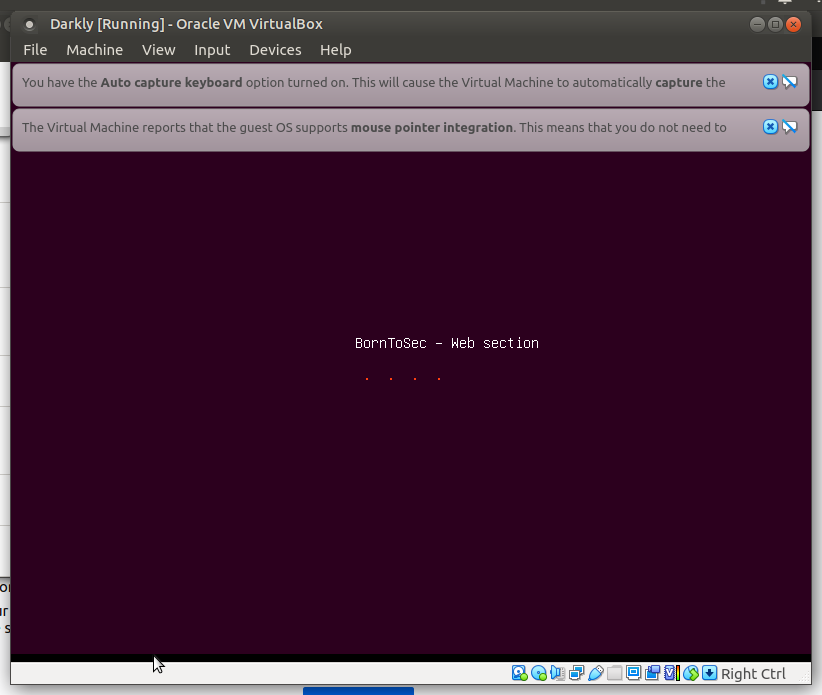
\includegraphics[width=0.752\textwidth]{images/00-12.png}\\[0cm]  
    \caption[Virtual Box]{\emph{Virtual Box Landing}, on Ubuntu}
    %from \url{http://localhost:3000/}).} % The text in the square bracket is the caption for the list of figures while the text in the curly brackets is the figure caption
    \label{fig:00-12 - Linux Virtual Box Landing} 
\end{figure}

Tell the system to use Linu
\subsubsection{Linux}

\begin{figure}[!htb]
    \centering
    %\insertcode{Scripts/example.pl}{Nena would be proud.} % The first argument is the script location/filename and the second is a caption for the listing
    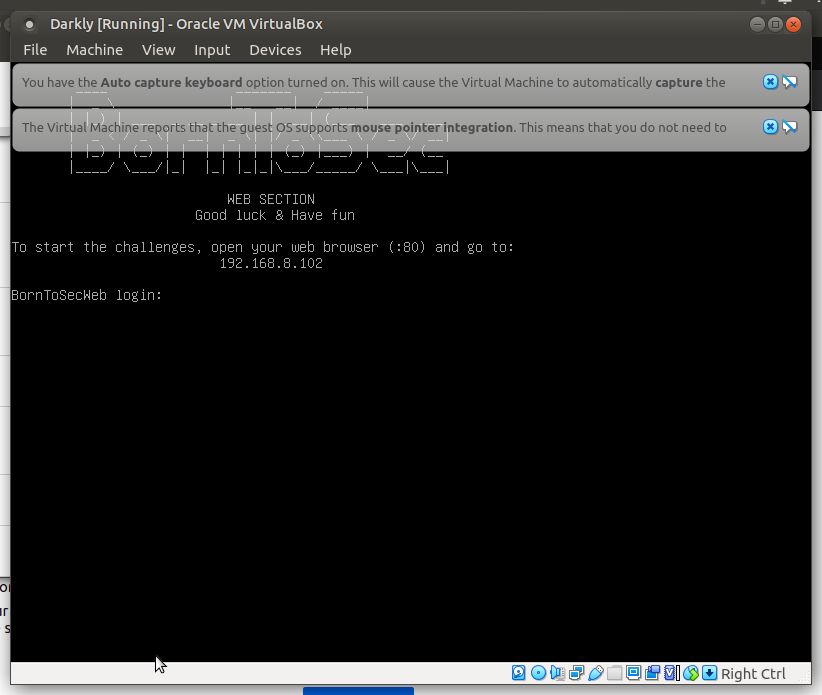
\includegraphics[width=0.752\textwidth]{images/00-13.png}\\[0cm]  
    \caption[Virtual Box]{\emph{Virtual Box Landing}, on Ubuntu}
    %from \url{http://localhost:3000/}).} % The text in the square bracket is the caption for the list of figures while the text in the curly brackets is the figure caption
    \label{fig:00-13 - Linux Virtual Box Landing} 
\end{figure}

Tell the system to use Linu
\subsubsection{Linux}

\begin{figure}[!htb]
    \centering
    %\insertcode{Scripts/example.pl}{Nena would be proud.} % The first argument is the script location/filename and the second is a caption for the listing
    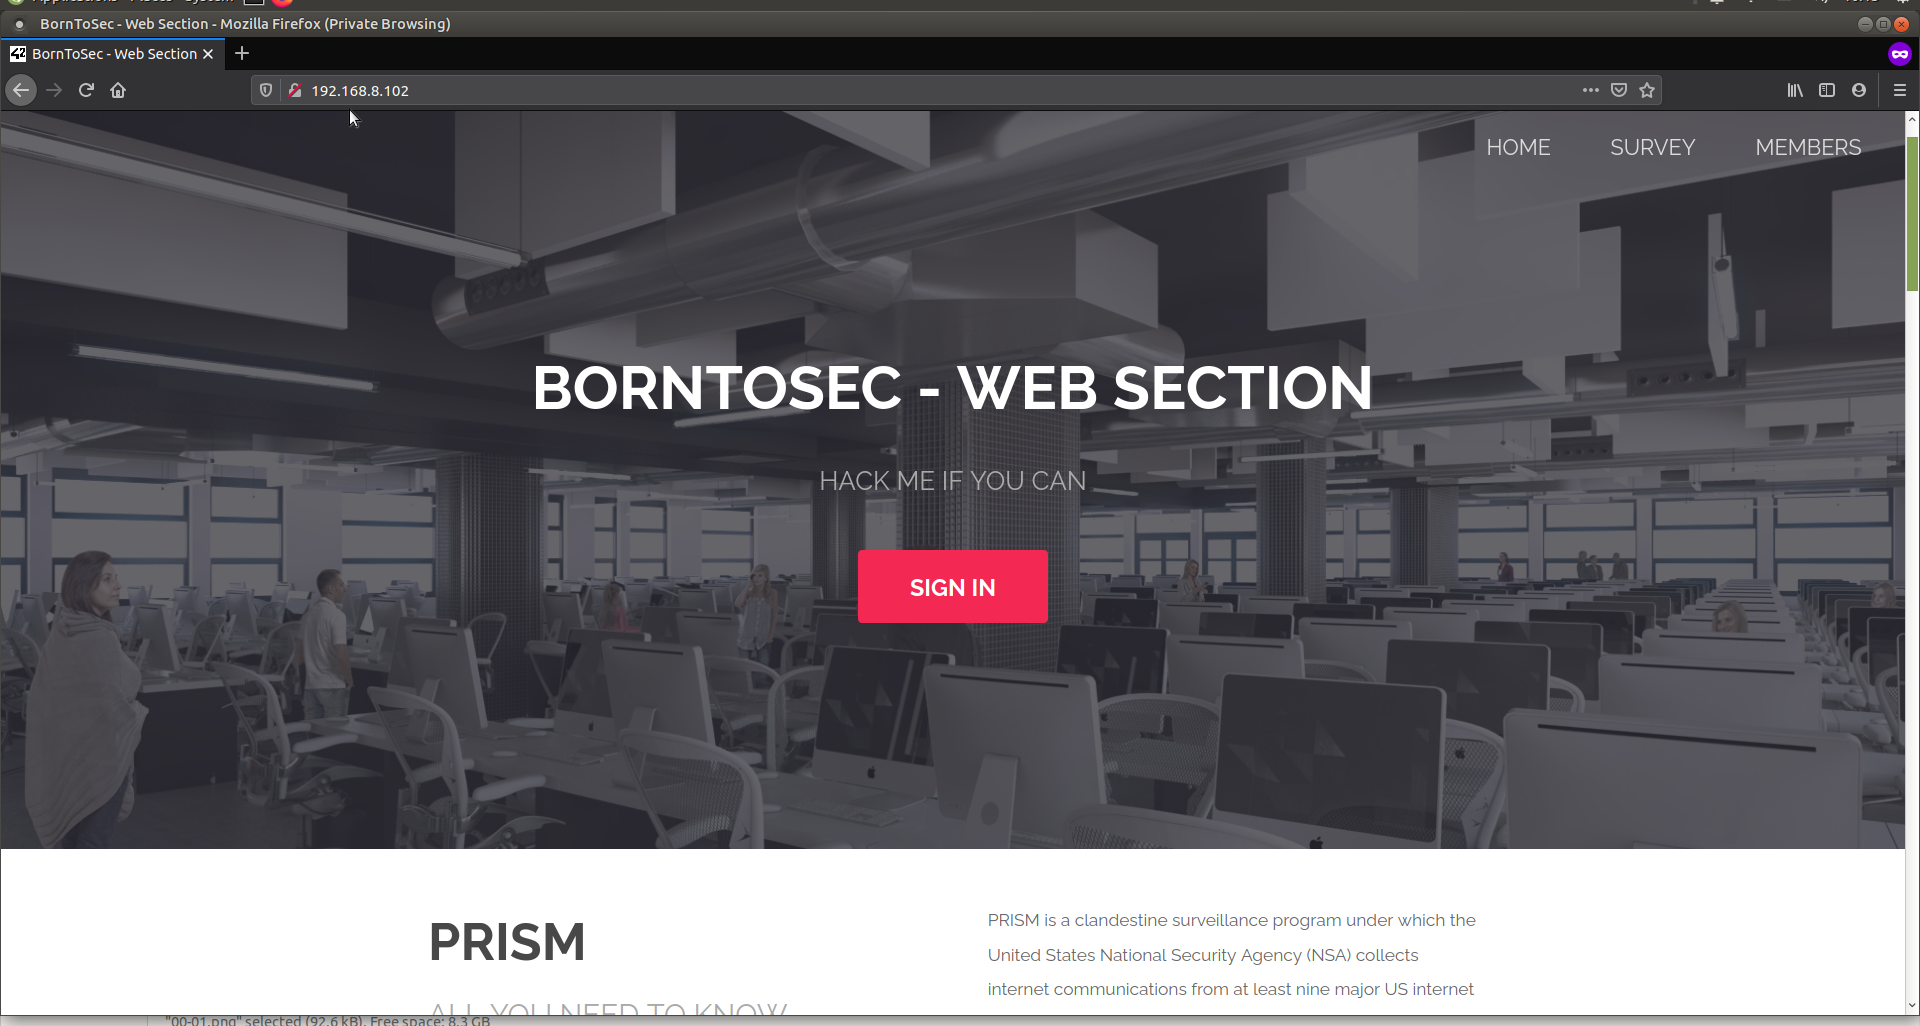
\includegraphics[width=0.752\textwidth]{images/00-14.png}\\[0cm]  
    \caption[Virtual Box]{\emph{Virtual Box Landing}, on Ubuntu}
    %from \url{http://localhost:3000/}).} % The text in the square bracket is the caption for the list of figures while the text in the curly brackets is the figure caption
    \label{fig:00-14 - Linux Virtual Box Landing} 
\end{figure}

Tell the system to use Linu
\clearpage
